\chapter{Prototipo 3: Obtener recomendaciones para diversos fines (sistemas híbridos)}
  \section{Análisis}
    \subsection{Objetivo}
      Generar las operaciones lógicas necesarias para realizar recomendaciones generalizadas para sistemas híbridos.

    \subsection{Características}
    \begin{itemize}
      \item El sistema proveerá las reglas, especificaciones y funciones necesarias para obtener recomendaciones de cualquier tipo de artículo que esté acorde al modelo propuesto.
      \item El sistema proveerá la funcionalidad de recomendaciones híbridas (basadas en contenido y colaborativas).
      \item El sistema proveerá los servicios necesarios para hacer posible la extensión de las funcionalidades desarrolladas.
    \end{itemize}

    \subsection{Restricciones}
    \begin{itemize}
      \item El sistema será capaz de obtener recomendaciones de artículos solo que empaten con el modelo propuesto. 
      \item El sistema será capaz de obtener recomendaciones de acuerdo a la funcionalidad desarrollada hasta el momento, siendo capaz de extender su funcionalidad a través de interfaces implementables.
    \end{itemize}

  \section{Diseño}
  Para la generalización de las recomendaciones sobre cualquier objeto acorde al modelo propuesto, se desarrollaron servicios basados en interfaces que permiten al desarrollador, utilizar la funcionalidad de la API, así como abstraer y modelar los objetos propios del sistema que desean desarrollar. 

  Para esto se utilizaron las interfaces Item, Characteristic y User, de las cuales las clases del dominio implementan para modelar cada uno de los comportamientos descritos para cada uno de los tipos de entidad identificados por las interfaces, permitiendo la obtención de los datos para el funcionamiento de la API y a su vez, la manipulación de los mismos en los procesos lógicos desarrollados en la API.

  Así mismo, para establecer las relaciones existentes entre estas entidades fue necesario establecer las interfaces Event, Neighbor y Affinity. Cada una de estas describe un comportamiento propio de las características de la relación. Como se puede ver en la figura~\ref{fig:p3_interfaces}, estas interfaces planteadas determinan el comportamiento de la API descrito en los párrafos posteriores, modelando las entidades y relaciones de la figura~\ref{fig:p3_general_model}

  \begin{landscape}
    \begin{figure}[h!]
      \centering
      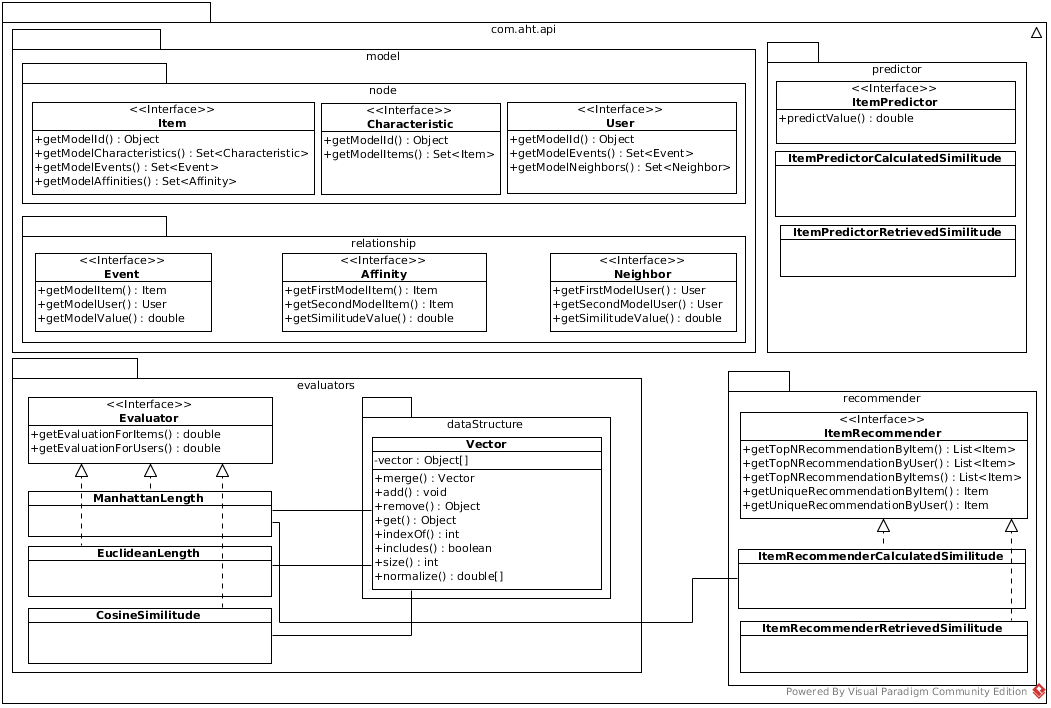
\includegraphics[width=24cm]{./images/classes_api}
      \caption{Diagrama de clases de la API}
      \label{fig:p3_interfaces}
    \end{figure}
  \end{landscape}

    \begin{figure}[h!]
      \centering
      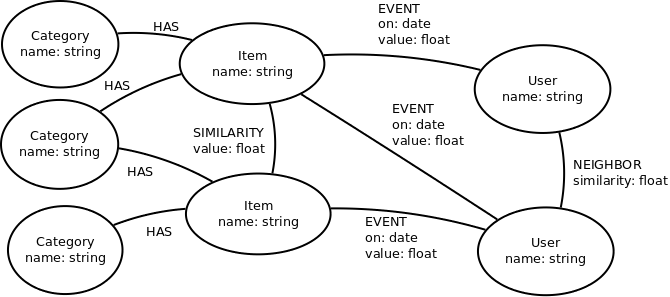
\includegraphics[width=16cm]{./images/general_data_model}
      \caption{Modelo generalizado de datos}
      \label{fig:p3_general_model}
    \end{figure}

  \subsection{Interfaces utilizadas para el modelo de entidades y relaciones}
    \paragraph{Item}
    Describe una entidad de tipo ítem. Estas entidades son el objetivo a recomendar por parte del sistema. Es decir, que el procesamiento lógico tiene como finalidad la recomendación de solo entidades de esta clase.

    \paragraph{User}
    Describe el comportamiento de una entidad de tipo usuario. Estas entidades son responsables de alimentar el sistema a través de su interacción con los artículos a recomendar. Gracias a dichas interacciones es posible obtener información paara generar recomendaciones.

    \paragraph{Characteristic}
    Describe una entidad de tipo característica. Este tipo de entidad permite la abstracción de características propias de las entidades de tipo \emph{Item}  que son determinantes para su categorización. Estas características fungen como un catálogo de los posibles valores existentes entre los diferentes tipos de artículos, gracias a la relación existente entre un \emph{Item} y sus características es posible llevar a cabo la recomendación basada en contenido.

    \paragraph{Event}
    Describe la relación existente entre un usuario y un ítem. Teniendo como propiedad un valor numérico que determina el peso de la relación, ya sea dada por un rating cuantitativo del usuario o por la cantidad de veces que el usuario ha tenido determinada interacción con el ítem.

    \paragraph{Affinity}
    Describe una relación entre dos ítems o artículos. Esta relación tiene como propiedad un valor de similitud determinado por una función de distancia o pseudo-distancia entre los mismos. Como resultado de esto, es posible determinar como objetivo la minimización de distancia o bien la maximización de similitud.

    \paragraph{Neighbor}
    Describe una relación entre dos usuarios registrados del sistema. Dicha relación se ve determinada por las interacciones entre usuarios e ítems, estas interacciones determinadas por los eventos de un usuario permiten a través del procesamiento de los datos, calcular una distancia o pseudo-distancia entre él y otros usuarios registrados, resultando en el valor para dicha relación. 

    Las interfaces descritas previamente permiten como resultado la manipulación de los datos de manera generalizada. 

  \subsection{Interfaces utilizadas para la recomendación y posible extensión de funcionalidad}
    Para realizar las recomendaciones, fue necesario tener diferentes servicios determinados por funciones de recomendación, de predicción y evaluadores para obtener las distancias o pseudo-distancias a utilizar. Para esto se planteó el uso de las interfaces \emph{ItemRecommender}, \emph{ItemPredictor} y \emph{Evaluator}.

    \paragraph{\emph{ItemRecommender}}
      Describe el comportamiento de la implementación de un algoritmo de recomendación que tiene como objetivo devolver un conjunto de ítems que representan una recomendación. Ejemplo de implementaciones son las clases \emph{ItemRecommenderGeneral} y \emph{ItemRecommenderNeo4j} las cuales describen la implementación de algoritmos para filtrado por contenido y filtrado colaborativo. \emph{ItemRecommenderGeneral} hace uso del modelo general sin relaciones de afinidad ni vecindad, y por su parte \emph{ItemRecommenderNeo4j} hace uso del modelo general dependiendo del mantenimeinto de las relaciones de afinidad y vecindad. 

    \paragraph{\emph{ItemPredictor}}
      Describe el comportamiento de un predictor de valores para un respectivo ítem o conjunto de ítems y un respectivo usuario. De esta manera, es posible determinar cuantitativamente un valor esperado u aproximado de una inexistente y tal vez futura relación entre un usuario y un ítem. Este valor es determinado por la similitud existente entre el ítem evaluado y el conjunto de ítems con los que un usuario ha interactuado previamente. Ejemplos de implementaciones se desarrollaron en \emph{ItemPredictorGeneral} e \emph{ItemPredictorNeo4j} 

    \paragraph{\emph{Evaluator}}
      Esta interfaz describe el comportamiento de las funciones de evaluación necesarias para calcular la distancia o pseudo-distancia entre dos items o usuarios. Este valor describe la diferencia o similitud con base en la distancia calculada, dependiendo del algoritmo de evaluación implementado. Ejemplo de clases que implementan esta interfaz son \emph{ManhattanLenght}, \emph{EuclideanLength} y \emph{CosineSimilitude}. 

    
  \section{Resultados}
    Para comprobar las funcionalidades de la API, se utilizaron las clases de dominio Dish, Characteristic y User las cuales implementan las interfaces de modelo para las entidades, descritas con anterioridad.

    Así mismo, se utlizaron las clases Affinity y Neighbor implementando las interfaces de modelo para las relaciones. Estas clases de dominio mapean los resultados del modelo de datos que se puede observar en la figura~\ref{fig:p3_db}

    \begin{figure}[h!]
      \centering
      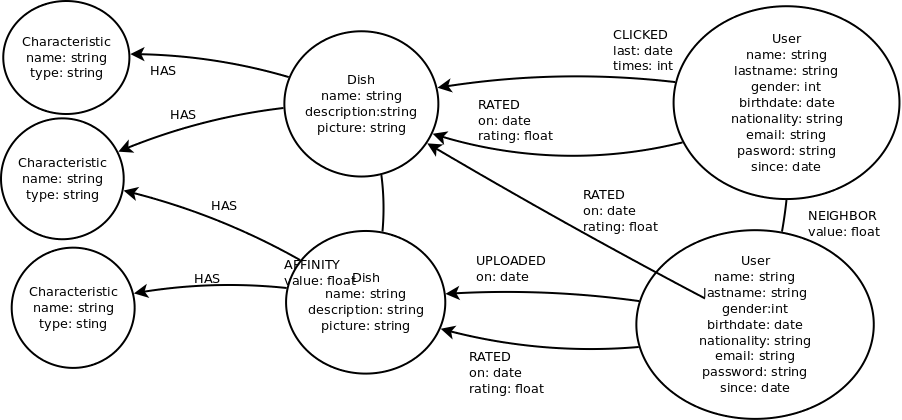
\includegraphics[width=16cm]{./images/p3_bd}
      \caption{Modelo de datos para el prototipo 3}
      \label{fig:p3_db}
    \end{figure}

    Utilizando las interfaces propuestas en la API, se crean las clases de dominio Dish, User y Characteristic para las entidades, así como Rate, Affinity y Neighbor para el modelado de las relaciones como se muestra en la figura~\ref{fig:p3_classes}

  \begin{landscape}
    \begin{figure}[h!]
      \centering
      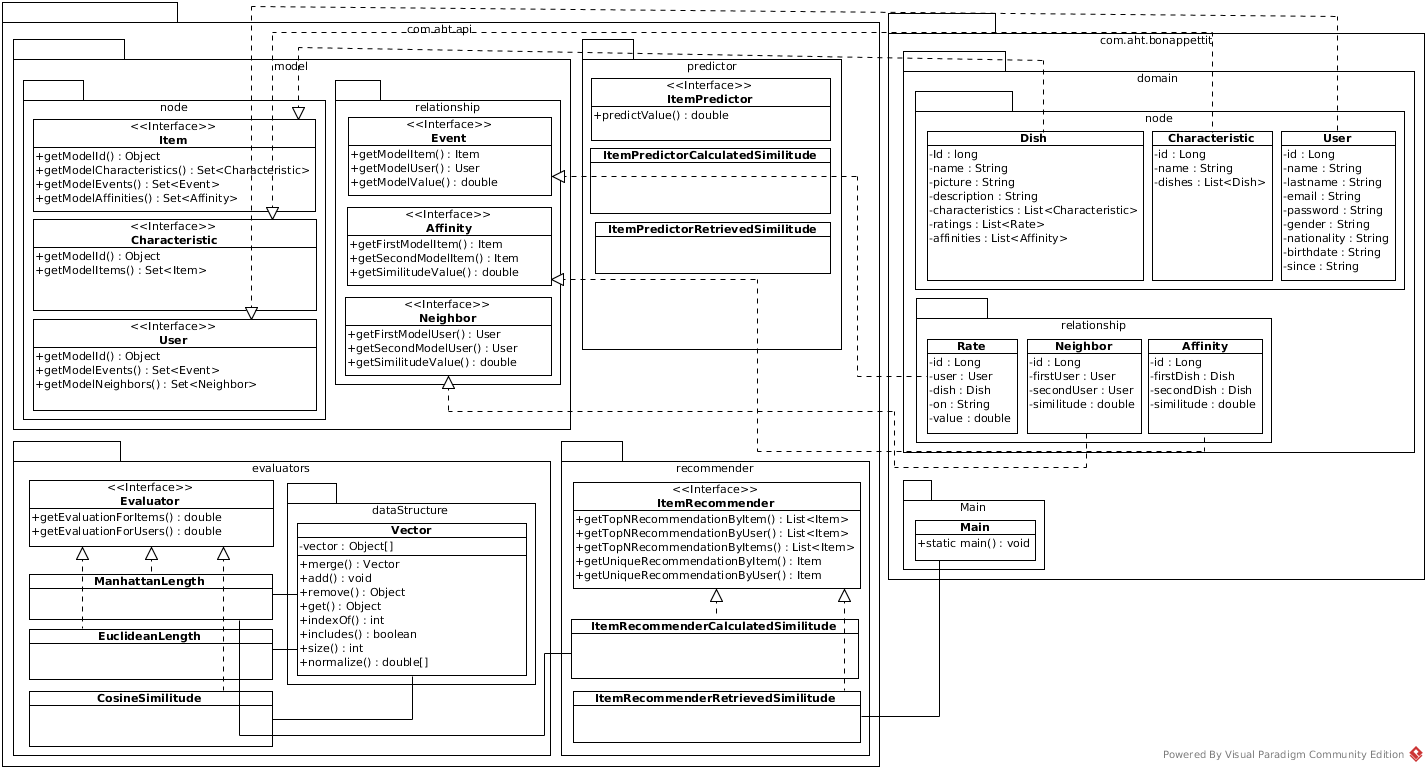
\includegraphics[width=25cm]{./images/p3_classes}
      \caption{Diagrama de clases del prototipo 3}
      \label{fig:p3_classes}
    \end{figure}
  \end{landscape}




